\section{Introduction}

\begin{figure}
  \centering
  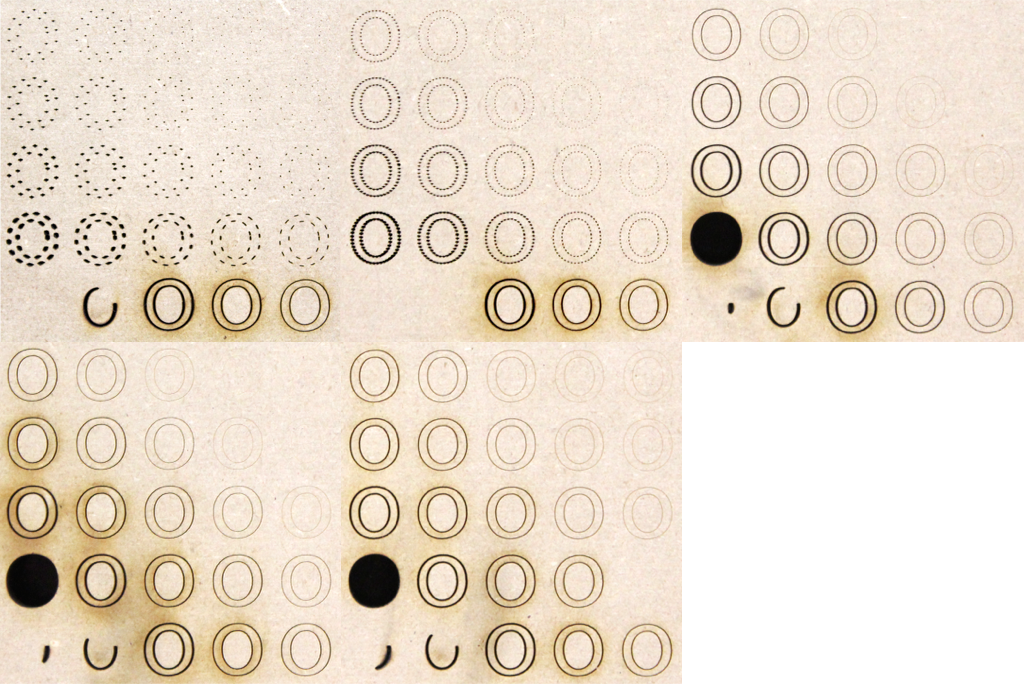
\includegraphics[width=0.4\textwidth]{figures/engravings}
  \caption{%
    A user of the laser cutter has to manipulate the laser's parameters to get the desired appearance.
    Black holes are when the laser passes completely through the material---
    the center is cut out and falls through.
  }\label{fig:rasters}
\end{figure}

\andrew{Make sure to tie this into what my contributions are to our class and what they should take away.}

This is a laser cutter---the VersaLaser 3.50.
It can do things like cut out shapes of materials, trace lines into material, and raster images.
It can do this with many different materials, like wood or acrylic.
But today, these are what the interfaces look like.
If you want to change the settings for vector cutting or engraving, you'll have to set these parameters here.
But it's not straightforward what all of them mean in terms of a firing laser beam. 
In the words of a pilot study participant when working with this type of interface for a few minutes, ``I still don't have a good mental model of how the heck this thing works.''

This is an engraving or a tracing---a laser has traced out an ``O'' on a piece of particle board I gave it.
There are tons of different ways we can engrave this O for different visual effects.

This project evaluate the human factors for a couple of algorithm-interface pairs to enable quick and enjoyable discovery of ``the right parameters''.
It focuses on a machine---a laser---that we can't really relate to by what our own bodies can do. 
And it focuses on comparison judgments because we need to make relative judgments, but humans are much better suited to making comparison judgments than singular ones.

To frame this problem in a way I could test it, I engraved this O with a bunch of different settings.
Then in a couple of interfaces, I showed people one of the Os as a goal, and a set of options that they had to rank.
For different ranking schemes, I change the front-end.
What are the pairs of algorithms and interfaces I use?

Consider what it takes to configure a laser cutter to engrave workpieces.
Consider the trivial ``O'' design in Figure~\ref{fig:rasters}.
Three parameters control the depth, speed, and resolution of the image etched into the material.
Improper values cause the image to appear only faintly, or scorch the material.

This research pursues a vision for fabrication machines that help users learn how to operate them.
My key insight is that the human factors of these algorithms can guide us to picking the right one for optimization.
Each configuration will comprise laser power, speed, frequency, and resolution.
The algorithm will suggest configurations and demonstrate them by rastering an image.
The algorithm will collect a user's rating of raster quality.
As the learned model will predict an continuous value, I will draw from past work for actively learning continuous-value models (e.g.~\cite{sugiyama_active_2008}).

To understand the trade-offs of this method of mixed initiative parameter space exploration, I ran a usability study.
This was on Mechanical Turk with 28 participants.
They were asked to recover a configuration for rastering an image that matches an exemplar I provide.
The method of parameter exploration was varied between two algorithms: Nelder-Mead~\cite{nelder_simplex_1964} and an instantiation of Bayesian optimization~\cite{brochu_tutorial_2010}.
I measured the total number of configurations tested, and Likert scale feedback on perceptions of the algorithms.
I also report on a pilot study that compares how people work with a standard slider-based interface for parameter exploration vs.\ and interface based on Nelder-Mead optimization.
